\documentclass[conference]{IEEEtran}
\usepackage[spanish,es-noshorthands,es-tabla]{babel}
\usepackage{amsmath}
\usepackage{graphicx}
\usepackage{booktabs}
\renewcommand{\tablename}{TABLA}
\renewcommand{\figurename}{Fig.}
\title{Del video de celular a la demostración para robot\\
Seguimiento de manos y detección de eventos de manipulación}
\author{
\IEEEauthorblockN{[Integrante 1], [Integrante 2], [Integrante 3]}
\IEEEauthorblockA{Proyecto final de Visión Artificial}
}
\begin{document}
\maketitle
\begin{abstract}
El seguimiento de manos en video RGB permite describir una demostración de manipulación mediante puntos articulares y eventos discretos. Se implementó un sistema para CPU que combina Hand Landmarker, preprocesamiento adaptativo, recuperación espacial y temporal, filtrado causal y una máquina de estados para detectar agarres y sueltas. El protocolo separa las tomas por secuencia, evalúa pose en píxeles y empareja eventos dentro de cinco cuadros. \input{build/resumen.tex} Las sueltas de DexYCB quedan fuera del protocolo. La evaluación con grabaciones propias y el evaluador de la asignatura determina el alcance de esta versión preliminar.
\end{abstract}
\begin{IEEEkeywords}
estimación de pose, seguimiento de manos, flujo óptico, agarre, video RGB
\end{IEEEkeywords}

\section{Introducción}
Una demostración manual observada con una cámara contiene trayectorias y cambios de estado que pueden servir como entrada para un sistema robótico. Para construir esa representación se necesita localizar la mano a lo largo del video y estimar cuándo entra y sale de contacto con un objeto. La proyección en una sola imagen pierde información de profundidad. Además, cuando la mano cubre el objeto, la evidencia visual puede reducirse precisamente en el intervalo donde ocurre el agarre.

La formulación de este proyecto conserva el problema en el plano de la imagen. Para cada cuadro produce el orden anatómico de 21 puntos de MediaPipe, y para cada transición emite un índice y una clase. La representación puede inspeccionarse en un video anotado y admite la entrada de una secuencia de imágenes. Este trabajo termina en la descripción de la demostración. Una aplicación robótica posterior tendría que resolver escala, pose y correspondencia con su actuador.

La comparación tiene dos objetivos. El primero es medir cobertura, exactitud espacial y estabilidad frente al modelo base. El segundo es medir la capacidad para ubicar agarres con una regla de tolerancia temporal. Estas metas están relacionadas: un error en las puntas de los dedos cambia la apertura estimada aunque se conserve una detección válida de muñeca.

\section{Trabajo relacionado}
DexYCB ofrece anotaciones de manos y objetos en secuencias sincronizadas \cite{chao2021dexycb}. Su adquisición multivista permite analizar la dificultad de observación y proporciona una trayectoria 3D del objeto para construir una referencia de agarre. La anotación de pose y la trayectoria sirven para evaluación. En la inferencia se utiliza la cámara RGB de entrada.

Pu et al. estudiaron exposición, desenfoque y oclusión mediante transformaciones controladas \cite{pu2023}. Reportaron que con desenfoque diagonal MediaPipe Hands dejó de localizar al menos la mitad de las manos de su protocolo. El hallazgo motiva analizar pérdida de detección y deterioro espacial por separado. El cambio de contraste puede ayudar en escenas oscuras, mientras que el flujo local requiere detalle espacial suficiente.

Chiche et al. mapearon landmarks a comandos de pinza e inverse kinematics de un brazo mediante una cámara egocéntrica RGB-D \cite{chiche2026}. El éxito estructurado fue de 86,7\,\% en su protocolo y descendió a 9,3\,\% en entornos no estructurados. La métrica mide ejecución del robot y depende de profundidad y calibración. Su experiencia ilustra la sensibilidad a oclusiones y el papel del suavizado de trayectorias.

El trabajo sobre contacto a escala de Internet separa pose de mano y estado de interacción con el objeto \cite{shan2020}. En esta implementación esa distinción motiva contrastar un cierre geométrico con movimiento visual de la vecindad. Esa evidencia local puede faltar en objetos uniformes y puede activarse ante movimiento de cámara.

\begin{figure}[t]
\centering
\setlength{\fboxsep}{3pt}
\begin{tabular}{c}
\fbox{\strut Video RGB o secuencia de imágenes}\\
$\downarrow$\\
\fbox{\strut Contraste adaptativo y realce opcional}\\
$\downarrow$\\
\fbox{\strut Hand Landmarker VIDEO en CPU}\\
$\downarrow$\\
\fbox{\strut Recuperación por ROI y flujo Lucas--Kanade}\\
$\downarrow$\\
\fbox{\strut Filtro causal de landmarks}\\
$\downarrow$\\
\fbox{\strut Geometría, evidencia RGB y estados}\\
$\downarrow$\\
\fbox{\strut puntos.csv y eventos.csv}
\end{tabular}
\caption{Flujo causal por cuadro. La evaluación utiliza anotaciones fuera de este flujo.}
\label{fig:pipeline}
\end{figure}

\section{Método de seguimiento}
El flujo de la Fig.~\ref{fig:pipeline} convierte BGR a RGB y se ejecuta cuadro por cuadro. Hand Landmarker utiliza la versión fijada del modelo y los umbrales de detección, presencia y seguimiento en 0,5 \cite{mediapipe}. El delegado de inferencia es CPU. La versión base conserva la salida directa de VIDEO. Las coordenadas se multiplican por el ancho y alto originales, y los timestamps se fuerzan a avanzar estrictamente en milisegundos.

\subsection{Fotometría y recuperación espacial}
Se estima iluminación a partir de luminancia. Se probaron gamma, ecualización global y CLAHE condicionado por iluminación. CLAHE calcula histogramas locales limitando la amplificación del contraste \cite{zuiderveld1994}. La transformación se aplica a luminancia, conservando crominancia. Gaussiano y bilateral reducen texturas de alta frecuencia. La máscara de enfoque añade una fracción de la diferencia entre la imagen y una versión gaussiana. El protocolo mide cuánto cambian las predicciones por cada opción y cuánto tiempo añade.

Cuando falla VIDEO, la ROI se centra en el último conjunto válido de puntos. El margen crece con el tamaño de la mano y el recorte se limita a la imagen. Se aplica Hand Landmarker en modo IMAGE al recorte. Para una coordenada normalizada $(u,v)$, el retorno a la imagen es $(x_0+u w_r,y_0+v h_r)$, con origen y tamaño de la ROI original. La ROI requiere una referencia reciente y se descarta tras una pérdida prolongada.

\subsection{Flujo óptico y suavizado}
Si falla la recuperación espacial, Lucas--Kanade piramidal propone desplazamientos locales entre dos cuadros \cite{lucas1981}. Se revisan los 21 puntos en ambas direcciones, se limita el error de parche, se descartan salidas de imagen y se comprueba plausibilidad métrica de las conexiones de la mano. El flujo se admite como máximo durante dos cuadros consecutivos. Si la evidencia es insuficiente se emite una fila con celdas vacías.

One Euro ajusta una frecuencia de corte en función de una velocidad filtrada \cite{casiez2012}. Para cada punto, $\alpha=\left(1+(2\pi f_c\Delta t)^{-1}\right)^{-1}$ y el aumento de $f_c$ con la velocidad reduce retraso durante movimientos rápidos. EMA utiliza un peso fijo. Kalman usa posición y velocidad con ruido de proceso, innovación y reinicio ante discontinuidades \cite{kalman1960}. Los filtros actualizan su estado con observaciones disponibles y se reinician tras un intervalo sin observaciones.

\section{Detección de eventos}
La apertura combina separaciones y flexión de dedos normalizadas por escala de palma. Un detector sencillo observa cierre y desaceleración. El detector propuesto emplea umbrales distintos para cierre y apertura, confirmación temporal y una duración mínima de agarre. El cuadro estimado corresponde al inicio de una transición confirmada posteriormente. La implementación guarda ambos índices durante la experimentación y exporta el inicio estimado.

La evidencia visual se calcula con puntos de interés alrededor de la mano y fuera de su vecindad inmediata. El desplazamiento local compatible con la trayectoria de la muñeca se contrasta con el movimiento estimado de fondo. La persistencia reduce oscilaciones entre estados cuando una medida cae cerca de un umbral. Un hueco breve tolera la pérdida de landmarks. Un hueco prolongado reinicia contadores y estado.

La rapidez se mide en relación con la escala de la mano para que un desplazamiento en píxeles tenga interpretación comparable entre distancias. Una proyección oblicua puede presentar poca variación de apertura durante un agarre real. También puede ocurrir el caso inverso cuando la mano libre se cierra. El tratamiento del contacto sigue siendo una inferencia por señales indirectas de RGB.

\section{Datos y protocolo experimental}
Se utilizó un prefijo verificado de las secuencias completas del sujeto 01 de DexYCB. Se conserva el identificador de la toma y se asignan juntas sus ocho cámaras mediante un hash determinista y una semilla registrada. Cada evaluación ligera utiliza la misma cámara preseleccionada en todas las tomas. Se conserva un piloto de desarrollo y se usa validación para seleccionar una configuración antes de leer las anotaciones de prueba.

El agarre de referencia se aproxima por el inicio de movimiento del objeto indicado por los metadatos de la toma. Se estima una pose inicial con cinco cuadros válidos y se busca una transición sostenida de al menos tres cuadros con 8\,mm de traslación o 12 grados de rotación. El consenso de cámaras evita atribuir un cambio a una anotación ruidosa aislada. Si las cámaras elegibles discrepan en más de cinco cuadros, la toma queda sin referencia de evento. DexYCB se evalúa únicamente en agarres en este protocolo.

Las tres condiciones propias previstas son buena luz, poca luz y movimiento rápido. Cada grabación debe contener cinco traslados con los cuadros de agarre y suelta anotados manualmente. El criterio temporal se aplica a ambas clases en dichas grabaciones. El modelo y los parámetros se conservan fijados al analizar videos nuevos.

\subsection{Métricas}
La detección se normaliza por cuadros con al menos una junta válida en imagen. PCK@10 px contabiliza las juntas de referencia válidas y marca una predicción ausente como fallo. El PCK condicional restringe el denominador a puntos emparejados y se usa como diagnóstico complementario. El temblor es la media de la norma de la segunda diferencia de posición en tríos consecutivos. Se incluyen aceleración de referencia y residuo para interpretar cambios asociados con el movimiento real. El número de tríos elegibles permite verificar que la cobertura no explique por sí sola una reducción.

Los eventos se emparejan del mismo tipo con tolerancia de $\pm5$ cuadros. Se maximiza la cardinalidad y se minimiza el error temporal absoluto en empates. El resultado incluye verdaderos positivos, falsos positivos y falsos negativos agregados por cuadro de evento y por vista independiente. El tiempo incluye lectura JPEG, extracción de landmarks y cómputo de eventos. Se registran recursos, versiones y hash del modelo por ejecución.

\section{Resultados}
\input{build/resultados.tex}
La diferencia de cobertura debe interpretarse junto al número de cuadros visibles. Una sola recuperación cambia una tasa de forma apreciable en un subconjunto pequeño. Las métricas de esta evaluación utilizan un sujeto y una cámara. Generalizar a teléfonos, personas y condiciones de iluminación diferentes requiere las grabaciones propias y más secuencias.

\section{Ablación y análisis de fallas}
\input{build/ablacion.tex}
La comparación de filtros examina el costo de amortiguar desplazamientos rápidos. Un descenso de la aceleración puede ir acompañado de un incremento del error espacial por rezago. La recuperación por flujo requiere consistencia de los parches. Cuando un dedo queda oculto o el objeto ocupa un parche, aceptar la predicción podría extender un error de identidad. Este diseño privilegia la evidencia de imagen y acota la duración de la recuperación.

\IfFileExists{figures/falla_dexycb.jpg}{
\begin{figure}[t]
\centering
\includegraphics[width=\columnwidth]{figures/falla_dexycb.jpg}
\caption{Cuadro de DexYCB seleccionado por ausencia de pose en un cuadro visible o por error mediano de al menos 15\,px en la vista comparada. Izquierda, MediaPipe. Derecha, sistema evaluado.}
\end{figure}
}{}
El detector distingue agarre y suelta por transiciones de apertura con persistencia. En el piloto aparecieron agarres con dedos extendidos en la proyección de la cámara. La apertura permaneció por encima del umbral absoluto aun después del inicio de movimiento del objeto. Esta limitación afecta la sensibilidad a agarres laterales y puede requerir una segmentación explícita o una referencia de movimiento más localizada.

\IfFileExists{figures/errores.png}{
\begin{figure}[t]
\centering
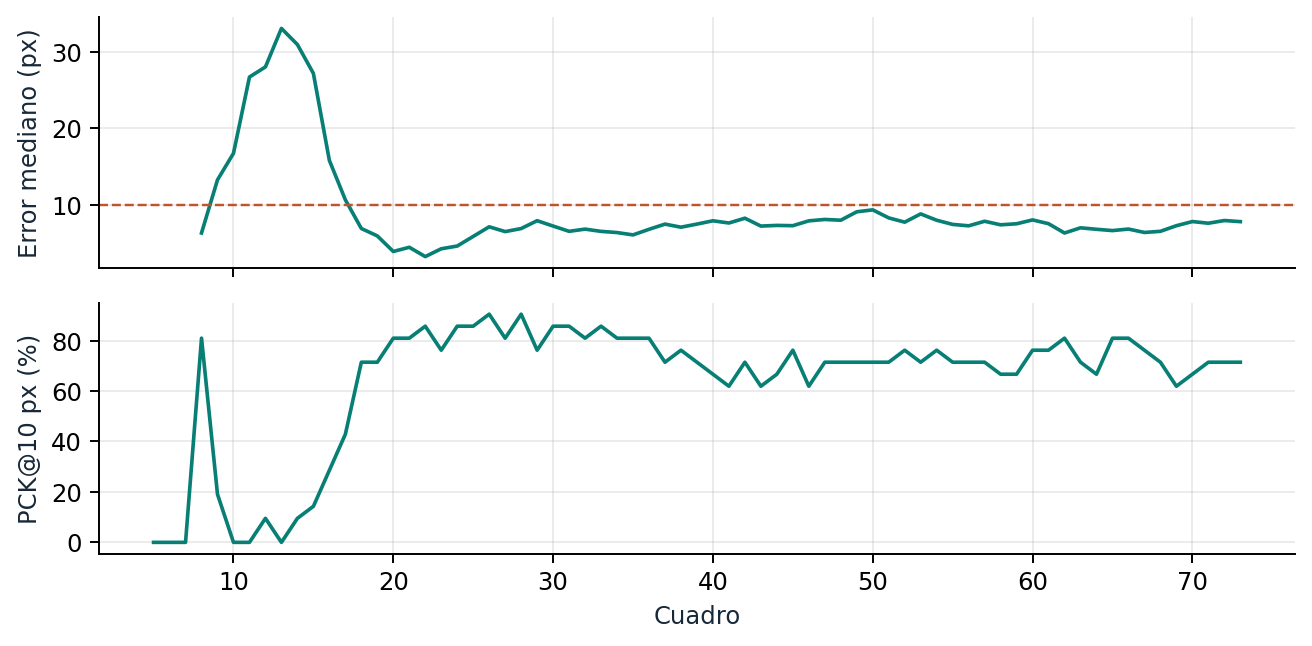
\includegraphics[width=\columnwidth]{figures/errores.png}
\caption{Error mediano y PCK de la vista del comparativo. Los huecos sin predicción quedan en blanco en la serie de error. El PCK cuenta las juntas de referencia perdidas como fallas.}
\end{figure}
}{}

\subsection{Casos de agarre y error espacial}
\input{build/casos.tex}
El filtro modifica posiciones en función de observaciones anteriores. El error de ese cuadro es compatible con un rezago, así como con errores de pose comunes a ambos métodos. La comparación de aceleración residual describe la diferencia temporal respecto a la referencia, pero un residuo menor puede coexistir con sesgo espacial.

\section{Discusión y conclusiones}
La salida en formato CSV conserva la cronología y una representación explícita de cuadros perdidos. La comparación utiliza el mismo modelo en ambos sistemas, con trazabilidad de las opciones añadidas. Las recuperaciones y el filtro modifican aspectos diferentes: cobertura en intervalos difíciles, continuidad de las trayectorias y precisión de puntos en movimiento. Analizar los tres ejes evita elegir un método basado únicamente en estabilidad.

El resultado de los eventos depende de la etiqueta aproximada de DexYCB y de la evidencia visible en una única cámara. Con pocos agarres, un acierto cambia sustancialmente F1. Los eventos propios permitirán comprobar si la lógica de suelta funciona y si el costo temporal de la confirmación es razonable. La versión preliminar entrega un flujo reproducible en CPU y conserva las variantes que permiten inspeccionar la contribución de cada técnica.

\bibliographystyle{IEEEtran}
\bibliography{references}
\end{document}
